\documentclass[11pt,a4paper]{article}
\usepackage[margin=1in]{geometry}
\usepackage{booktabs}
\usepackage{graphicx}
\usepackage{hyperref}
\usepackage{amsmath}
\usepackage{float}
\usepackage{caption}
\graphicspath{{figures/}{./figures/}{./}}

\title{AI651 -- Deep Learning for Space, Time and Graphs\\Assignment 1 Report}
\author{Osama Atiq}
\date{\today}

\begin{document}
\maketitle

\noindent\textbf{GitHub repository (public):}
\url{https://github.com/OsamaAtiq12/DL4STG-PA1}

\section{Task 1 -- Forecasting Across Heterogeneous Sensors}

From a context of $L{=}96$ samples we forecast $H{=}48$ vibration readings (20\,Hz). Stations~1--3 are established; Station~4 is held out. Products A/B/C run at different paces.

\subsection{Response 1A -- Ordering of forecasters}
\textbf{Before Output 1.1} I expected
\[
\text{Period-routed ridge}
\;\succ\;
\text{Raw Attention}
\;\succ\;
\text{Shared ridge}
\;\succ\;
\text{Sensor-specific ridge}
\]
on established stations, and the same on Station~4 except that sensor-specific ridge cannot be scored there (no Station~4 weights).

\textbf{After Output 1.1} (validation RMSE, $m/s^2$):

\begin{center}
\begin{tabular}{lcc}
\toprule
Model & Established & Held-out \\
\midrule
Period-routed ridge & \textbf{0.166} & \textbf{0.173} \\
Raw Attention & 0.431 & 0.612 \\
Shared ridge & 0.767 & 0.876 \\
Sensor-specific ridge & 0.768 & --- \\
\bottomrule
\end{tabular}
\end{center}

The measured order matches the prediction. Period routing wins on both populations because it conditions on operating pace. Shared and sensor-specific ridge are nearly tied on established stations; Raw Attention beats both but stays behind period routing.

\subsection{Response 1B -- Why the rule must depend on context}
Output~1.2 (Station~1): Product~A has period ${\approx}16.1$ and Product~C has period ${\approx}30.1$. Shared ridge RMSE is $0.779$ (A) and $0.448$ (C); period-routed ridge drops to $0.232$ and $0.150$. One fixed shared matrix cannot handle both paces, so it compromises.

Output~1.3: the same Attention projections give different mixing weights across those two contexts (mean $|\Delta w|{=}0.011$, max $0.425$). That is context-dependent mixing, not recovery of the true period. The forecasting rule must depend on the current window.

\begin{figure}[H]
\centering
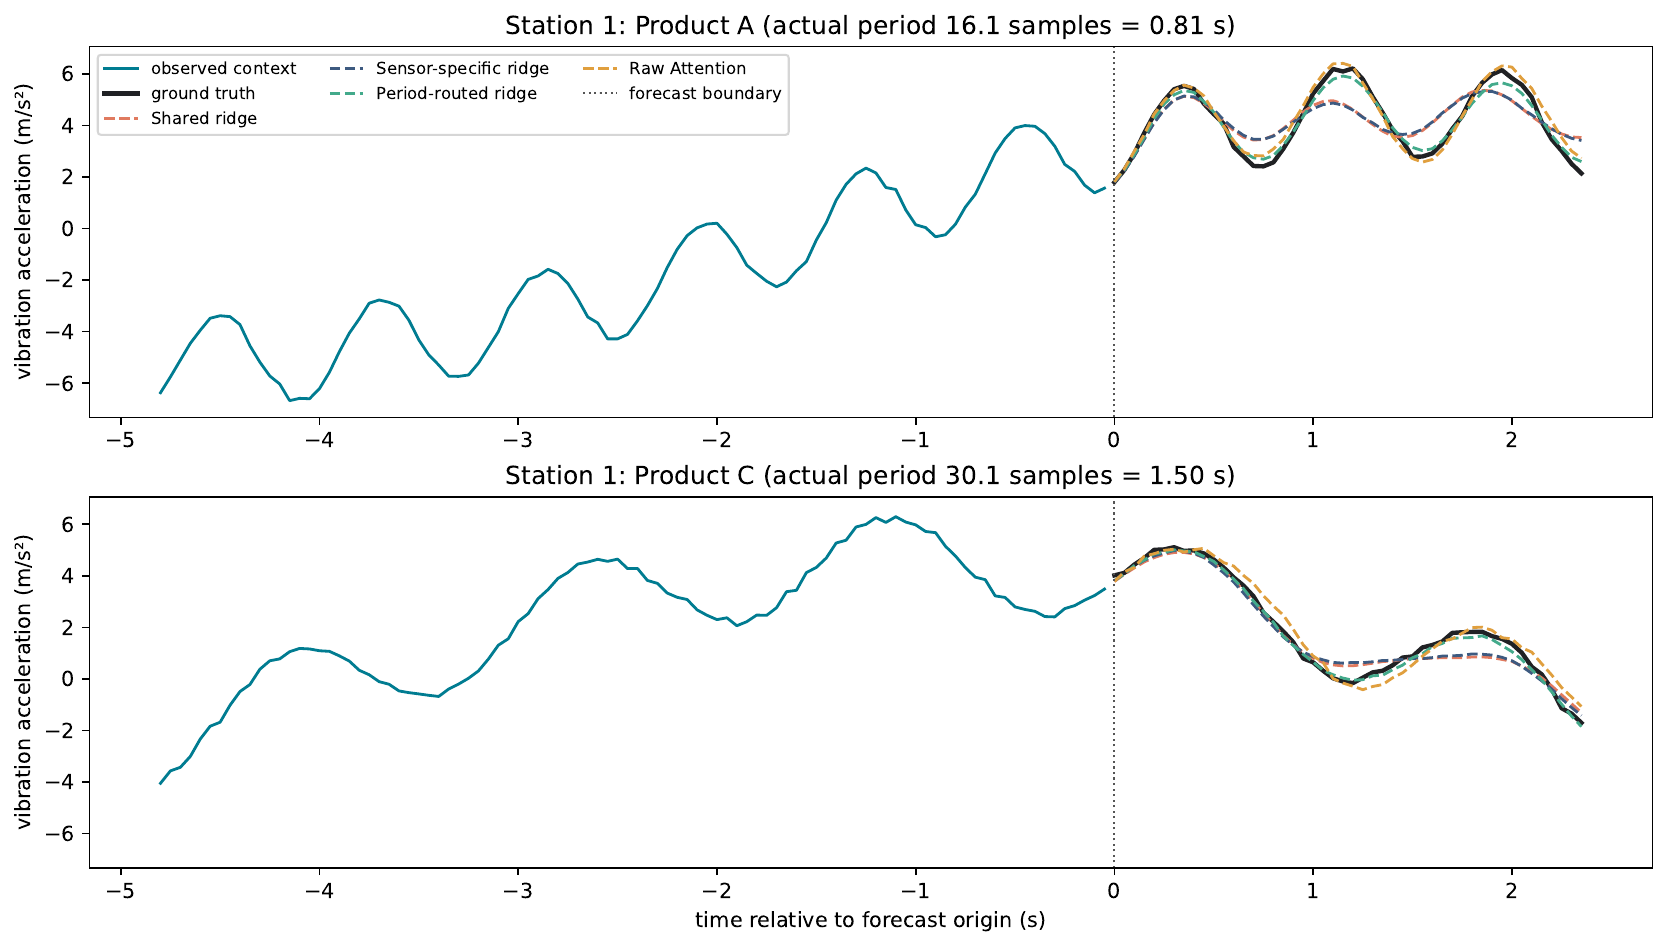
\includegraphics[width=0.95\textwidth]{1.2-1.png}
\caption{Output 1.2: same station, two products.}
\end{figure}

\begin{figure}[H]
\centering
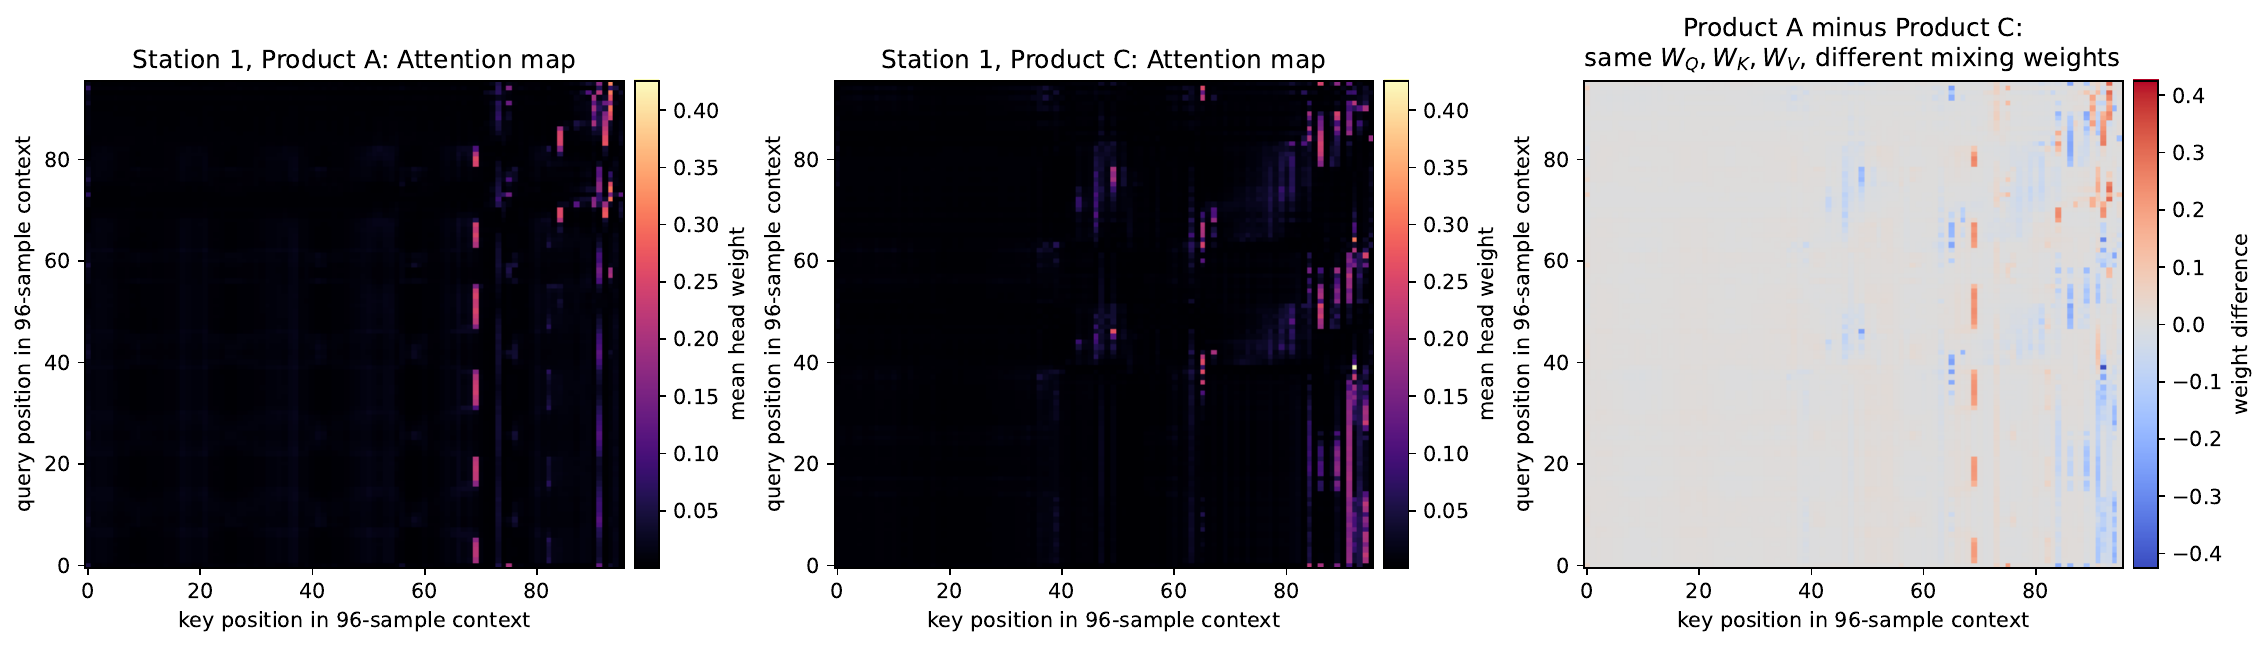
\includegraphics[width=0.95\textwidth]{1.3-1.png}
\caption{Output 1.3: Attention weight differences across contexts.}
\end{figure}

\subsection{Response 2 -- Decomposition}
Selected width: \textbf{41} (Outputs~2.1--2.2). It gives the best oracle period recovery within one sample ($0.998$ vs.\ $0.687$ on the raw signal). A centered moving average is a sensible bias here because the slow drift changes more slowly than the $14$--$36$ sample vibration cycle, so a fixed smoother can peel trend from residual before mixing. Output~2.3 shows decomposition also lowers Attention RMSE (e.g.\ established Product~A: $0.388\to0.264$).

Failure case: a sudden level jump or strong curvature inside one window can be mis-split by a fixed-width average. An alternative is a learned / causal trend head with adaptive bandwidth.

\begin{figure}[H]
\centering
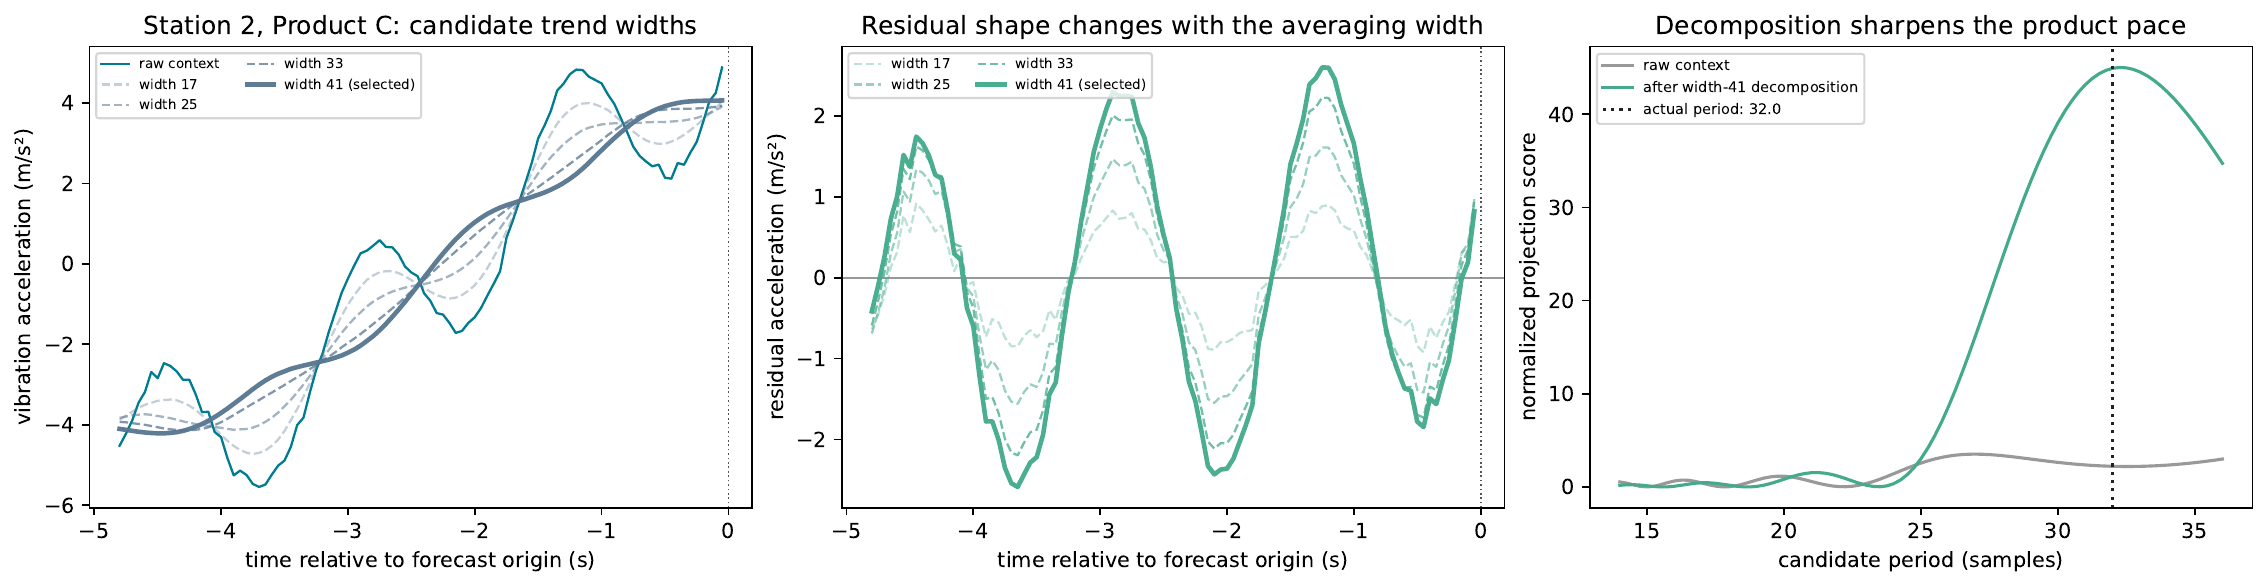
\includegraphics[width=0.95\textwidth]{2.1-1.png}
\caption{Output 2.1: candidate widths.}
\end{figure}

\begin{figure}[H]
\centering
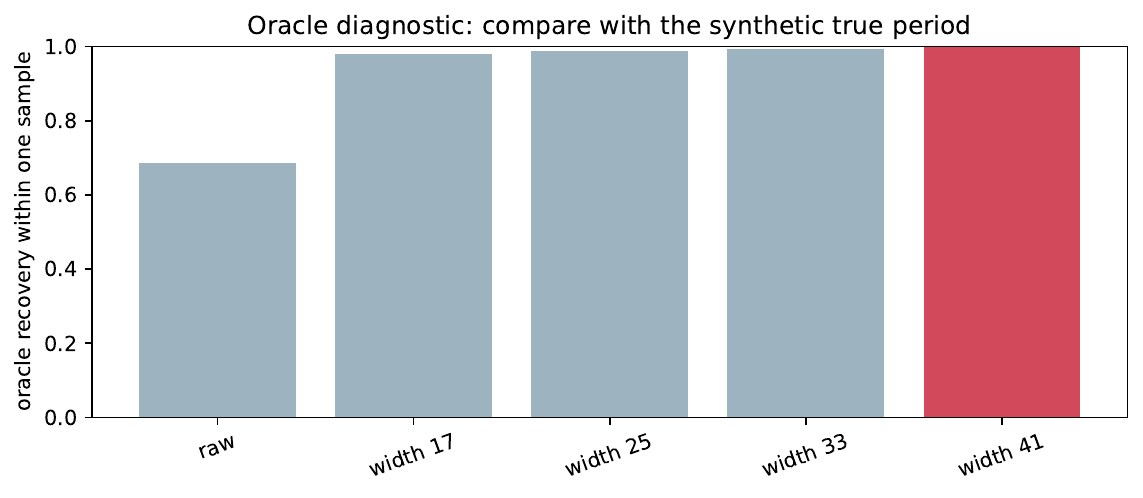
\includegraphics[width=0.95\textwidth]{2.2-1.png}
\caption{Output 2.2: oracle period recovery.}
\end{figure}

\begin{figure}[H]
\centering
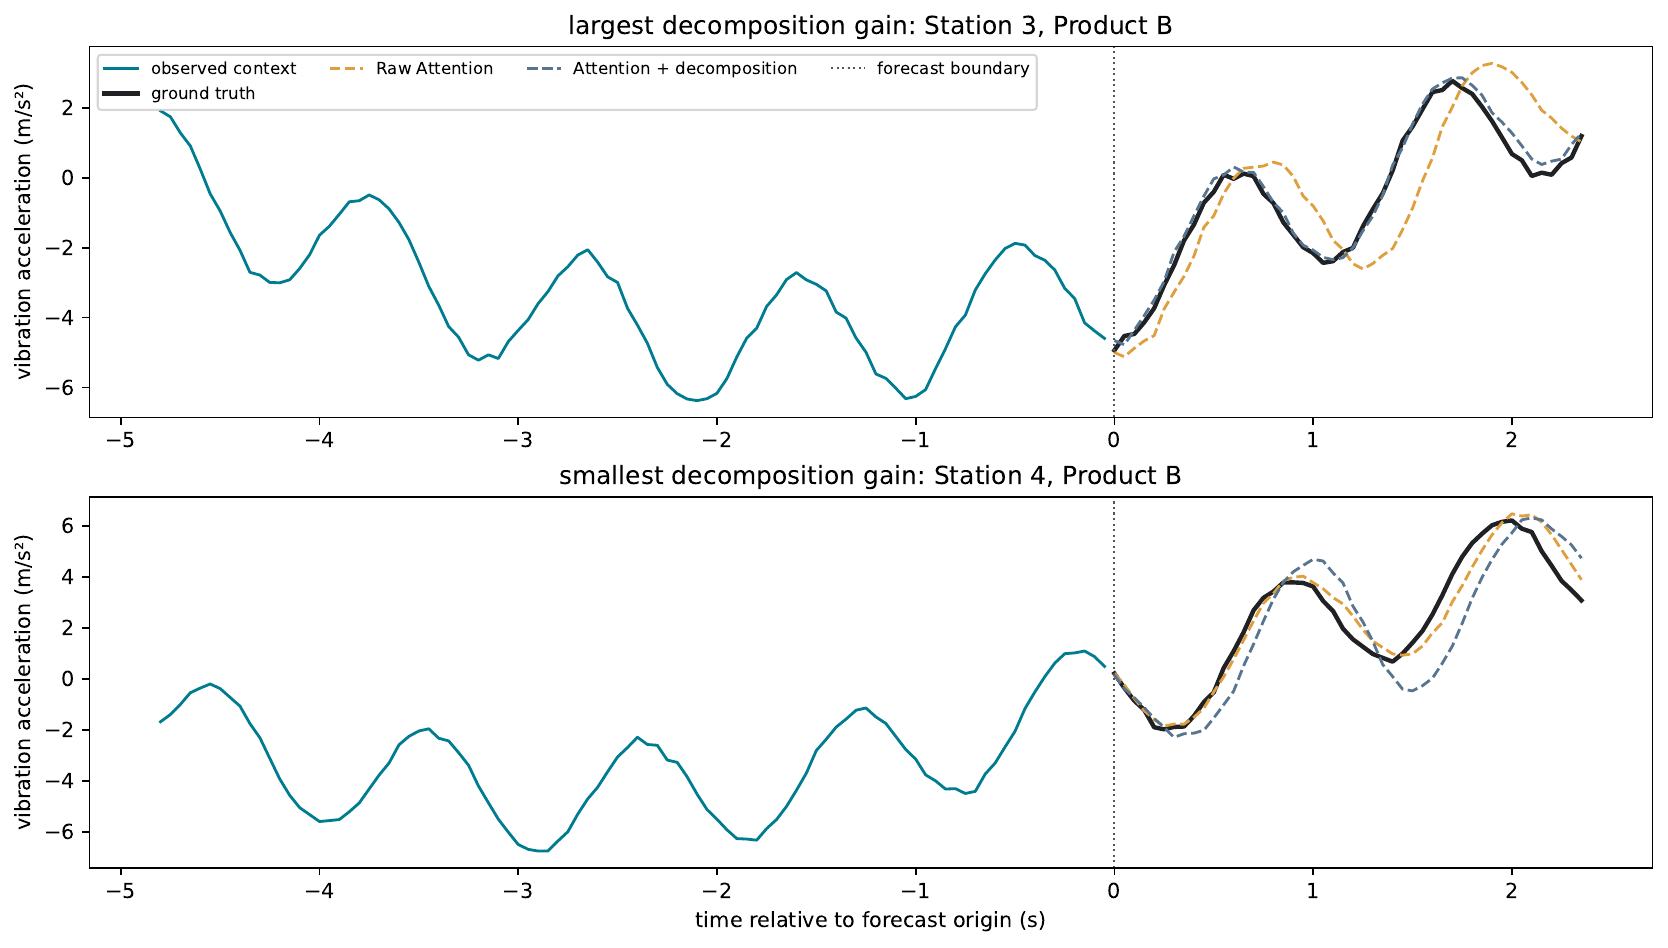
\includegraphics[width=0.95\textwidth]{2.3-1.png}
\caption{Output 2.3: Attention with vs.\ without decomposition.}
\end{figure}

\subsection{Response 3 -- Delay mixing}
Output~3.2 (Product~A, $P{\approx}16.13$): strongest residual correlations are at delays $16$ and $32$ (${\approx}0.896$), i.e.\ $P$ and $2P$. After removing the slow component these peaks are clearer, so delay mixing has cleaner evidence. Output~3.1 checks that FFT delay scores match direct circular correlation.

Delay mixing is the wrong bias for an aperiodic transient or a period that drifts inside one $L{=}96$ window, because top-$K$ lag aggregation would mix mismatched histories.

\begin{figure}[H]
\centering
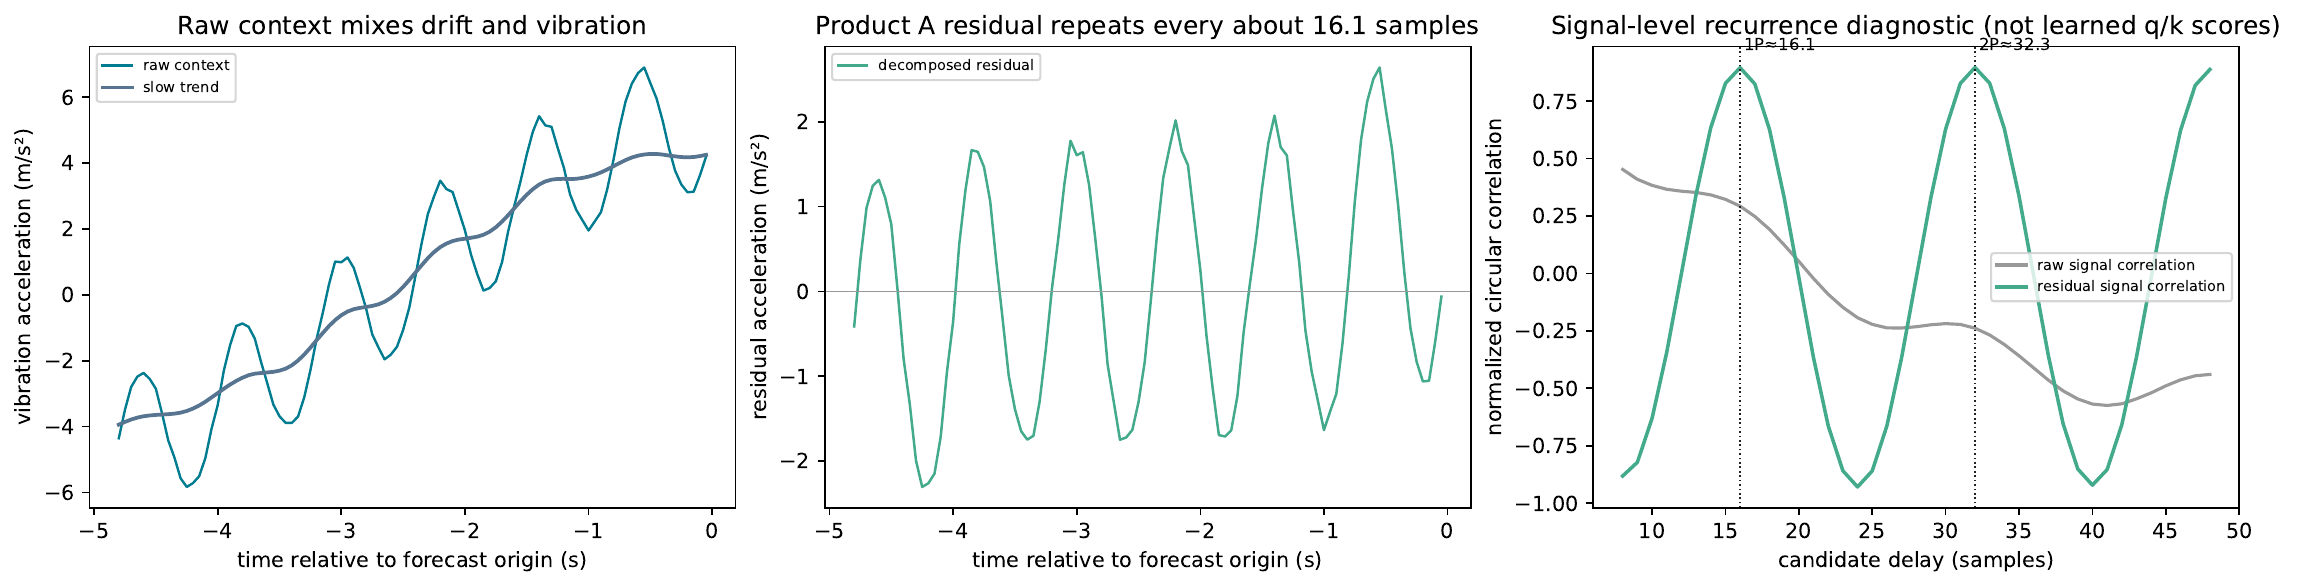
\includegraphics[width=0.95\textwidth]{3.2-1.png}
\caption{Output 3.2: recurrence diagnostic.}
\end{figure}

\subsection{Response 4 -- Compare and deploy}
\textbf{(a) Before Output 4.1.} When the slow component is strong, I expected decomposition to help most: the trend head takes the ramp and the mixer sees a cleaner residual.

\textbf{(b) Output 4.1--4.2.} Among neural configs, Autoformer-inspired is best on established stations (RMSE $1.832$), then Raw Attention ($1.884$), Raw delay mixer ($1.985$), Attention$+$decomposition ($2.081$). On Station~4, Raw Attention is slightly best among neural models ($1.995$). Combining both switches is not uniformly better than Attention alone. Horizon error grows with lead time (Output~4.2). Period-routed ridge is still far stronger and cheaper (Output~1.1: $0.166$ / $0.173$).

\begin{figure}[H]
\centering
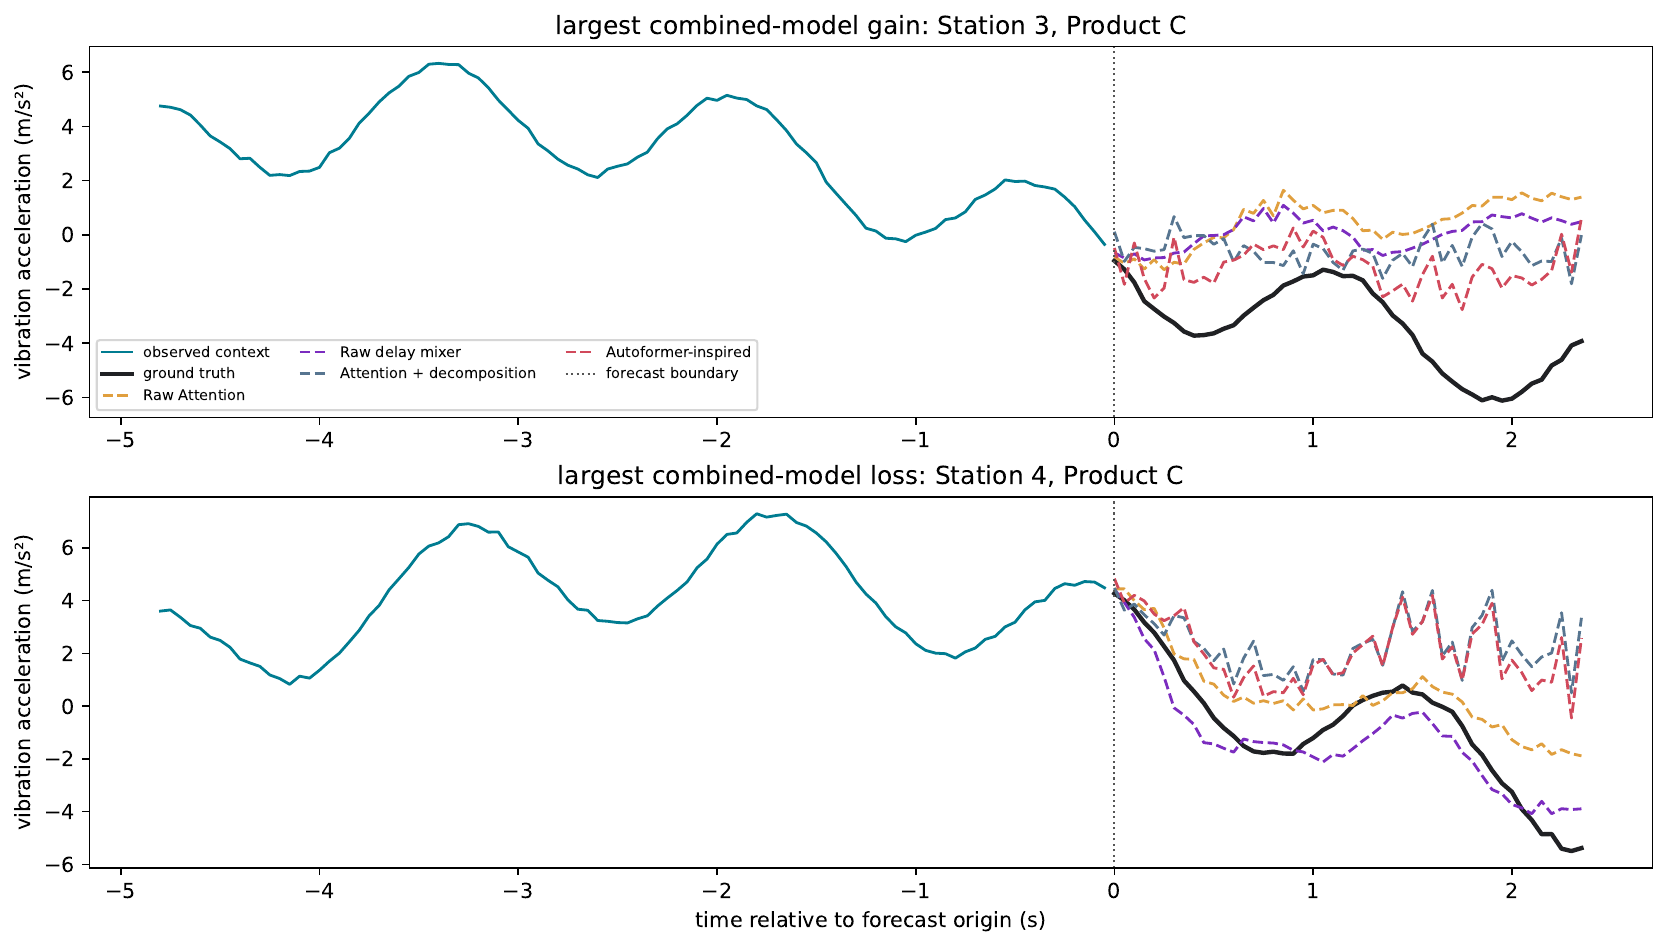
\includegraphics[width=0.95\textwidth]{4.1-1.png}
\caption{Output 4.1: neural comparison.}
\end{figure}

\begin{figure}[H]
\centering
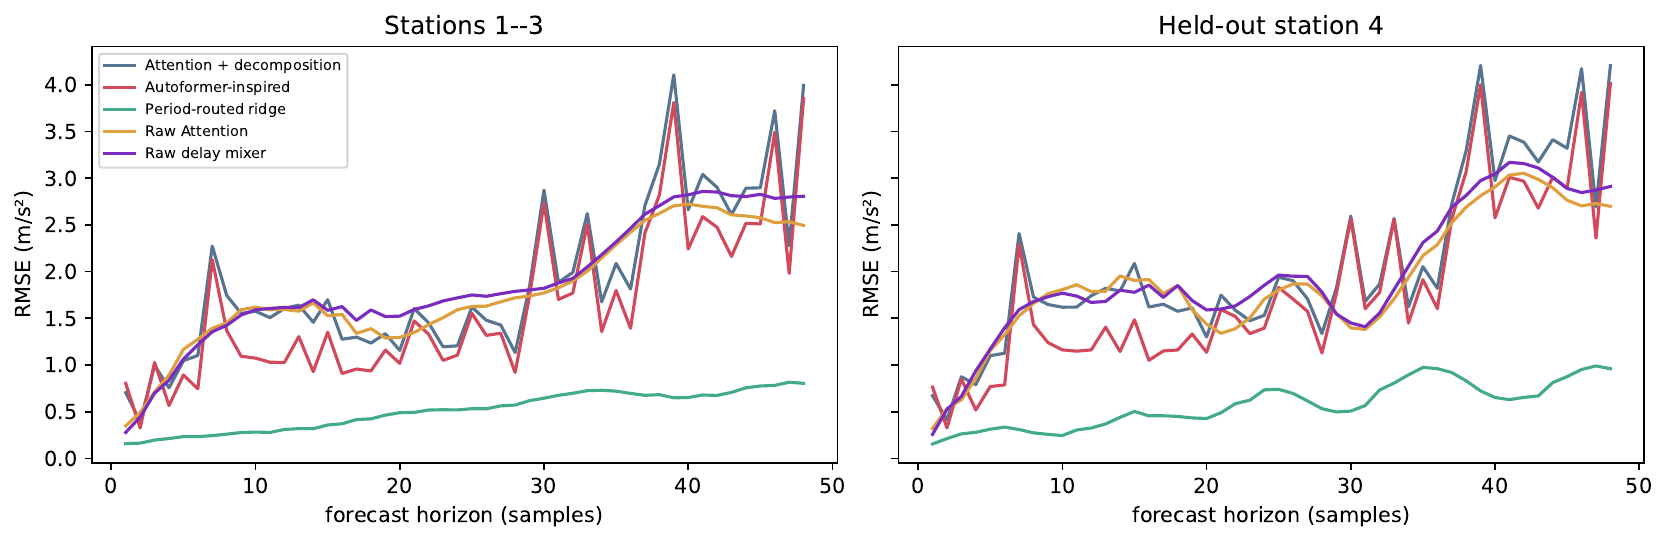
\includegraphics[width=0.95\textwidth]{4.2-1.png}
\caption{Output 4.2: horizon-wise error.}
\end{figure}

\textbf{(c) Deployment.}

\begin{center}
\begin{tabular}{lll}
\toprule
Population & Model & Reason \\
\midrule
Established & Period-routed ridge & Best val RMSE/MSE, low cost \\
Held-out Station 4 & Period-routed ridge & Best held-out RMSE \\
\bottomrule
\end{tabular}
\end{center}

Output~4.3 test RMSE: established $0.643$; held-out $0.753$.

\section{Task 2 -- Leaderboard Challenge}

Compact Autoformer (decomposition + Auto-Correlation / delay aggregation): context $336$, label $84$, horizon $168$, $d{=}32$, one encoder/decoder layer; AdamW; two seeds; final forecast averages the seeds after a short full-history refit.

Best validation RMSE:

\begin{center}
\begin{tabular}{lcc}
\toprule
Setting & Seed 0 & Seed 1 \\
\midrule
Without external features & 94.83 & 95.70 \\
With external features & \textbf{62.06} & \textbf{64.07} \\
\bottomrule
\end{tabular}
\end{center}

External features help, so the submission uses them. Declared $P{=}46532$, $E{=}6$.

\section*{AI Policy Compliance}
Tools used: GitHub Copilot was used for code completion, syntax assistance, and concept understanding. All final code, numbers, and written Responses were checked and edited by me.

\end{document}
